\documentclass{article}
\usepackage{amsmath}
\usepackage{amsfonts}
\usepackage[english]{babel}
\usepackage[utf8]{inputenc}
\usepackage{amsthm}
\usepackage{graphicx}

\newcommand{\norm}[1]{\left\lVert#1\right\rVert}
\newtheorem{theorem}{Theorem}
\newtheorem{prop}{Proposition}
\newcommand{\overbar}[1]{\mkern 1.5mu\overline{\mkern-1.5mu#1\mkern-1.5mu}\mkern 1.5mu}

\begin{document}

\setlength\arraycolsep{2pt}
\title{Discontinous Galerkin Method for 1D Advection Equation}
\author{}
\maketitle


\section{Weak Formulation}
  
\noindent The problem that we want to solve is:

\begin{gather*}
  \frac{\partial u}{\partial t} + a \frac{\partial u}{\partial x} - bu = 0 \qquad x \in [-1, 1] \\
  u(0, t) = g(t) \\
  u(x, 0) = f(x) \\
\end{gather*}

\noindent We want to find $u_h$ that is an approximation of $u$, and $u_h = \bigoplus_{k=1}^K u_h^k$, where $k$ indexes elements. If we define the spaces $V$ and $V_f$ , $V_f^k$:

\begin{gather*}
  V = \{ v(x) : \norm{v}^2 < \infty, \langle v, v^{\prime}\rangle < \infty\} \\
  V_f = \{ v(x) : v \in V, v \text{ is a linear combination of basis functions}\} \\
  V_f^k = \{ v(x) : v \in V_f, x \in D^k\}\\
\end{gather*}

\noindent Where $D^k$ is the domain of element k.  We can now consider the error between  $u_h^k \in V_f^k$ and $u^k$. We get:

\begin{gather*}
  u_h^k - u^k = \left(\frac{\partial u_h^k}{\partial t} + a \frac{\partial u_h^k}{\partial x} - bu_h^k\right) - \left(\frac{\partial u^k}{\partial t} + a \frac{\partial u^k}{\partial x} - bu^k\right) = \\
  \left(\frac{\partial u_h^k}{\partial t} + a \frac{\partial u_h^k}{\partial x} - bu_h^k\right) - 0 = \frac{\partial u_h^k}{\partial t} + a \frac{\partial u_h^k}{\partial x} - bu_h^k \\
\end{gather*}

\noindent Similar to the Continious Galerkin (CG) Method we multiply the error by a test function and integrate, except now in Discontinious Galerkin (DG) the integral is over each element rather than the entire physical domain so that we get:

\begin{gather}
  \int_{D_k} \left(\frac{\partial u_h^k}{\partial t} + a \frac{\partial u_h^k}{\partial x} - bu^k_h\right) v dx = 0 \qquad \forall v \in V_f^k,  k \in K
\end{gather}

\noindent Where $K$ is the set of all elements on our domain. Also note that due to the definition of $V$ this equations makes sense (the integral is finite), and that while $u$ is both spatially dependent and time dependent, $v$ is only a function of space.

\vspace{3mm}

\noindent What is the best way to think about Eq. 1? Eq. 1 is saying that the error of what will be our solution is orthogonal to every function in $V_f^k$. From linear algebra we know that if $\left(\frac{\partial u_h^k}{\partial t} + a \frac{\partial u_h^k}{\partial x} - bu_h^k\right) \neq \vec{0}$, and it is orthogonal to every vector in $V_f^k$ then $\left(\frac{\partial u_h^k}{\partial t} + a \frac{\partial u_h^k}{\partial x} - bu_h^k\right) \notin V_f$.

\vspace{3mm}

\noindent The analog in $\mathbb{R}^n$ goes like this:

\noindent Let $e_i$ be the standard basis in $\mathbb{R}^n$, and
$\vec{u} \in \mathbb{R}^n$ such that $\vec{u} \cdot \vec{v} = 0, \forall v \in \mathbb{R}^n$. Then we can write:

$$\vec{u} \cdot \vec{v} = (a_1e_1)\cdot(b_1e_1) + (a_2e_2)\cdot(b_2e_2) + ... + (a_ne_n)\cdot(b_ne_n) = 0 \qquad \forall b_i \in \mathbb{R}$$

The only way we can zero out each term is if $a_i = 0$ otherwise there will be a nonzero $b_i$ leading to a nonzero term. $a_i = 0$ then implies that $\vec{u} = 0$.

\vspace{3mm}

\noindent In other words Eq. 1 is ``saying'' the error on a single element is not in our finite dimensional space $V_f^k$, or that the error in $V_f^k$ must be 0.

\section{System of Linear equations}

\noindent Further confining ourselves to the space:

$$ V_0^k = \{ v : v \in V_f^k, v \text{ is linear}\}$$

\noindent the problem becomes find $u_h \in V_0^k$ such that:

\begin{gather}
  \int_{D_k} \left(\frac{\partial u_h^k}{\partial t} + a \frac{\partial u_h^k}{\partial x} - bu_h^k\right) v dx = 0 \qquad \forall v \in V_0,  k \in K
\end{gather}

\noindent We can write (2) using a basis for $v$. Let $\phi_1$ and $\phi_2$ be lagragian basis functions on any element $k$, where:

\begin{gather*}
  \phi_1(x) = - \frac{x_r^k - x}{h}\\
  \phi_2(x) = \frac{x - x_l^k}{h}\\
\end{gather*}

Where $ h = x_r^k - x_l^k$, and $x_r^k$ is the $x$ value of the right side of the element, and $x_l^k$ is the left side.  Then (2) is equivalent to:

\begin{gather}
\int_{D_k} \left(\frac{\partial u_h^k}{\partial t} + a \frac{\partial u_h^k}{\partial x} - bu_h^k\right) \phi_i dx = 0 \qquad i = 1,2,  k \in K
\end{gather}

To see that (2) if and only if (3), first both equations for each element in (3) are just cases of (2) where if we write $v$ as a linear combintation of basis functions $v = v_1\phi_1 + v_2\phi_2$, we have $v_1 = 0$ for one case and $v_2 = 0$ for the other. On the other hand if (3) is true then multiplying through by a constant, and adding the two equations of (3) we recover (2).


Next, since $u_h \in V_0$ we can also write it as a combination of the basis functions on a single element so that:


$$u^k_h = \sum_{j=1}^2 \overbar{u}^k_j(x_j^k, t)\phi_j(x)$$

\noindent Where $\overbar{u}$ is a coordinate. It is important here to realize what we will be solving for in the long run. The basis functions are only functions of space like the test functions were. The coordinates of the basis functions are functions of time though, and at each timestep we want to solve for a new set of coordinates. Secondly the notation $ \overbar{u}^k_j(x_j^k, t)$ is not great, $x^k_j$ does not mean that $\overbar{u}^k_j$ is a function of space (their locations do not very in time), but only that this coordinate has an associated point on $x$, because the basis functions are interpolating polynomials. Plugging in this representation of $u_h^k$ to (3) we get:

\begin{gather*}
 \sum_{j=1}^2 \frac{\partial\overbar{u}^k_j}{\partial t}\int_{D_k}\phi_j\phi_i dx + a\sum_{j=1}^2 \overbar{u}^k_j\int_{D_k} \phi_j^{\prime} \phi_i dx - b  \sum_{j=1}^2 \overbar{u}^k_j\int_{D_k}\phi_j \phi_i dx = 0 \qquad i = 1,2,  k \in K
\end{gather*}

\noindent At this point we could make a systems of equations for each element, but there would be no connection between any of the elements, and no way for boundary data to enter the system. Doing integration by parts on the second term solves this problem, giving:

\begin{gather*}
  \sum_{j=1}^2 \frac{\partial\overbar{u}^k_j}{\partial t}\int_{D_k}\phi_j\phi_i dx + af^*\phi_i\biggr\rvert_{x_l^k}^{x_r^k}  - a\sum_{j=1}^2 \overbar{u}^k_j\int_{D_k} \phi_j \phi_i^{\prime} dx - b  \sum_{j=1}^2 \overbar{u}^k_j\int_{D_k}\phi_j \phi_i dx = 0 \qquad i = 1,2,  k \in K\\
\end{gather*}

\noindent Where instead of taking the boundaries of the element, we replace them with fluxes $f^*$. This is one of the really centeral pieces to DG. The DG user then defines what their flux is with their problem in mind (with convergance in mind too). We then integrate by parts again, to get SAT or penalty parameter terms for the boundaries of each element, so that we have:

\begin{gather*}
  \sum_{j=1}^2 \frac{\partial\overbar{u}^k_j}{\partial t}\int_{D_k}\phi_j\phi_i dx
  + af^*\phi_i\biggr\rvert_{x_l^k}^{x_r^k} -  au_h^k\phi_i\biggr\rvert_{x_l^k}^{x_r^k} + a\sum_{j=1}^2 \overbar{u}^k_j\int_{D_k} \phi_j^{\prime} \phi_i dx - b  \sum_{j=1}^2 \overbar{u}^k_j\int_{D_k}\phi_j \phi_i dx = 0 \qquad i = 1,2,  k \in K\\
\end{gather*}


\noindent Writing this in matrix form we get:
\begin{gather}
 M^k \frac{\partial\vec{u}_h^k}{\partial t} + a S^k \vec{u}_h^k - bM^k\vec{u}_h^k = (au_h^k(x_r^k) -af^*_r)\vec{\phi}(x_r^k) - (au_h^k(x_l^k) - af^*_l)\vec{\phi}(x_l^k)\qquad \forall k \in K\\
  M^k = \langle \phi_j, \phi_i \rangle \qquad S^k = \langle \phi_j^{\prime}, \phi_i\rangle
\end{gather}

\noindent The only thing left to figure out to have a linear system of equations is what the fluxes can and should be. For each adjacent element we have that $x^{k-1}_r = x^k_l$ and $x^k_r = x^{k+1}_l$ so that on each element boundary $u_h$ is multiply defined. So, the solution vector has length $2|K|$. It therefore seems reasonable to make each flux/penalty parameter be equal to some weighted average of values defined on element $k-1$ and element $k$ for the left boundary, and $k$ and $k+1$ for the right boundary, so that:

\begin{gather*}
  f^*_l = \alpha u_h^{k-1}(x^{k-1}_r) + (1-\alpha)u_h^k(x^k_l)\\
  f^*_r = \alpha u_h^{k}(x^{k}_r) + (1-\alpha)u_h^{k+1}(x^k_l)\\
\end{gather*}

Where $0 \leq\alpha \leq 1$. To include the physical boundary condtions, on the left side of the first element we can make $f^*_l = g(t)$, and at the right boundary we have no $k+1$ element so $f^*_r = u_h^k(x_r^k)$.

\section{Stability for Fluxes}

To find the stability conditions for the flux we can use the energy method. Similar to SBP-SAT we want $S^k$ to mimic summation by parts and $M^k$ to mimic the energy. Before showing this though the energy over the whole domain without any estimates is:

\begin{gather*}
  \frac{\partial}{\partial t} \norm{u}^2 =  \frac{\partial}{\partial t} \int_{-1}^1 u^2 dx = \int_{-1}^1 2u\frac{\partial u}{\partial t} dx = \int_{-1}^1 2u\left(bu-a\frac{\partial u}{\partial x}\right) dx = 2b\int_{-1}^1 u^2 dx - 2a\int_{-1}^1 u\frac{\partial u }{\partial x} dx \\
  =  2b\int_{-1}^1 u^2 dx - a\int_{-1}^1 u\frac{\partial u }{\partial x} dx + a\int_{-1}^1 u\frac{\partial u }{\partial x} dx - au^2\biggr\rvert_{-1}^1 = 2b\norm{u}^2 + a(u^2(-1) - u^2(1))
\end{gather*}

\newpage

\noindent To mimic this with $M^k$, and $S^k$ we have:

\begin{gather*}
  (\vec{u}_h^k)^T M^k \vec{u}_h^k =
  \begin{bmatrix}
    \overbar{u}_1^k && \overbar{u}_2^k \\
  \end{bmatrix}
  \begin{bmatrix}
    \int_{D^k} \phi_1 \phi_1 &&  \int_{D^k} \phi_1 \phi_2\\
    \int_{D^k} \phi_2 \phi_1 &&  \int_{D^k} \phi_2 \phi_2\\
  \end{bmatrix}
  \begin{bmatrix}
    \overbar{u}_1^k\\
    \overbar{u}_2^k \\
  \end{bmatrix}\\
  = \begin{bmatrix}
  \int_{D_k} \sum_{j=1}^2 \overbar{u}_1^k \phi_j \phi_1 &
  \int_{D_k} \sum_{j=1}^2 \overbar{u}_2^k \phi_j \phi_2 \\
  \end{bmatrix}
  \begin{bmatrix}
    \overbar{u}_1^k\\
    \overbar{u}_2^k \\
  \end{bmatrix}
  =  \norm{u_h^k}^2 \\
\end{gather*}
\begin{gather*}
  (\vec{u}_h^k)^T S^k \vec{u}_h^k =
    \begin{bmatrix}
    \overbar{u}_1^k && \overbar{u}_2^k \\
  \end{bmatrix}
  \begin{bmatrix}
    \int_{D^k} \phi_1 \phi_1^{\prime} &&  \int_{D^k} \phi_1 \phi_2^{\prime} \\
    \int_{D^k} \phi_2 \phi_1^{\prime} &&  \int_{D^k} \phi_2 \phi_2^{\prime}\\
  \end{bmatrix}
  \begin{bmatrix}
    \overbar{u}_1^k\\
    \overbar{u}_2^k \\
  \end{bmatrix}\\
  \begin{bmatrix}
  \int_{D_k} \sum_{j=1}^2 \overbar{u}_1^k \phi_j \phi_1^{\prime} &
  \int_{D_k} \sum_{j=1}^2 \overbar{u}_2^k \phi_j \phi_2^{\prime} \\
  \end{bmatrix}
  \begin{bmatrix}
    \overbar{u}_1^k\\
    \overbar{u}_2^k \\
  \end{bmatrix}
   = \int_{D_k} u_h^k\frac{\partial u_h^k}{\partial x} dx = \frac{1}{2} (u_h^k)^2\biggr\rvert_{x_l^k}^{x^k_r}
\end{gather*}

\noindent If we multiple (4) by $(\vec{u}^k_h)^T$, and move all of the terms to the right then we can get an energy estimate for the discrete system:

\begin{gather*}
  \frac{\partial}{\partial t}\norm{u_h^k}^2 = b\norm{u_h^k}^2 - a \frac{1}{2} (u_h^k)^2\biggr\rvert_{x_l^k}^{x^k_r} + \vec{u}_h^k\vec{\phi}(x_r^k)(au_h^k(x_r^k) - af^*_r) -  \vec{u}_h^k\vec{\phi}(x_l^k)(au_h^k(x_l^k) - af^*_l)\\
  = 2b\norm{u_h^k}^2 - a (u_h^k)^2\biggr\rvert_{x_l^k}^{x^k_r} + 2 u_h^k(x_r^k)(au_h^k(x_r^k) - af^*_r) - 2u_h^k(x_l^k)(au_h^k(x_l^k) - af^*_l)\\
  = 2b\norm{u_h^k}^2 + (a(u_h^k)^2(x_r^k) - 2u_h^k(x_r^k)af^*_r) - (a(u_h^k)^2(x_l^k) - 2u_h^k(x_l^k)af^*_l)
\end{gather*}

\noindent For our scheme to be stable we need $\frac{\partial}{\partial t}\norm{u_h^k}^2 \leq 0$ over the whole domain. We can ignore the expotential growth term (since unless $b \leq 0$ we know this will grow our solution). It is confusing to try to figure out global stability though in terms of local solutions. If we plug in our fluxes here, we will have terms involving $u^{k-1}$ and $u^{k+1}$. A way around this is to shift our persective from each element to each boundary between elements. If we define $u^- = u^{k-1}_r$ as the value on the boundary of the left element, and $u^+ = u^k_l$ as the value on the boundary of the right element. Then we need on every boundary:

\begin{gather*}
   a(u^-)^2 - 2(u^-)af^{-*} - a(u^+)^2 + 2(u^+)af^{+*} \leq 0\\
\end{gather*}

\noindent Plugging in the fluxes we get:

\begin{gather*}
  a(u^-)^2 - 2u^-a(\alpha u^- + (1-\alpha)u^+) - a(u^+)^2 + 2u^+a(\alpha u^- + (1-\alpha)u^+)\leq 0\\
  (a -2 a \alpha)(u^-)^2 - 4\alpha u^+ u^- + 2u^+u^- + (2a(1- \alpha) - a)(u^+)^2 \leq 0\\
\end{gather*}

Which is only stable for $ \frac{1}{2} \leq \alpha \leq 1$


\section{Local and Global Matrices}

The local scheme (rewriting equation 4 by dividing my $M^{-1}$) looks like this:

\begin{gather}
  \frac{\partial\vec{u}_h^k}{\partial t} =  (-a M^{-1} S^k) \vec{u}_h^k + b\vec{u}_h^k +  M^{-1}((au_h^k(x_r^k) - f^*_r)\vec{\phi}(x_r^k) - (au_h^k(x_l^k) - f^*_l)\vec{\phi}(x_l^k))\qquad \forall k \in K
  \end{gather}

Assuming we can integrate all the combintations of basis function that we need on a reference element then scale them to each element, we don't need anymore matrices. Since:

$$
\vec{\phi}(x_l^k) =
\begin{bmatrix}
  \phi_1(x_l^k) \\
  \phi_2(x_l^k) \\
\end{bmatrix}
= \begin{pmatrix}
  1 \\
  0 \\
\end{pmatrix}
$$

and the reverse for $\vec{\phi}(x_r^k)$, along with the expressions for the flux (6) becomes:

\begin{gather*}
\frac{\partial\vec{u}_h^k}{\partial t} =  (-a M^{-1} S^k +bI) \vec{u}_h^k +  M^{-1}F\vec{u}_h^{k{\prime}}
\qquad \forall k \in K \\
F = \begin{bmatrix}
  a\alpha & -a\alpha & 0 & 0 \\
  0 & 0 & a(1-\alpha) & -a(1-\alpha) \\
\end{bmatrix}\\
\vec{u}_h^{k\prime}=
\begin{bmatrix}
  u_r^{k-1} \\
  u_l^k \\
  u_r^k \\
  u_l^{k+1} \\
\end{bmatrix}\\
\end{gather*}

Constructing the global matrix, the RHS becomes a diagonal single banded matrix, with a vector for the boundary condition:

$$\frac{\partial\vec{u}_h^k}{\partial t} = G\vec{u}_h + b\qquad b = \begin{bmatrix} aM_{11}g(t)\\  aM_{21}g(t) \\ 0 \\ 0\\ \vdots \\ 0 \end{bmatrix}$$

\newpage

\section{Time Stability}

\noindent Using Euler to discretize in time, we can derive the region of absolute stability by inserting the test equation $\frac{\partial\vec{u}}{\partial t} = \lambda I \vec{u}$ into the foward Euler method:

\begin{gather*}
  \vec{u_n} = \vec{u}_{n-1} + k \frac{\partial\vec{u}}{\partial t} = \vec{u}_{n-1} + k\lambda I \vec{u}_{n-1} = (\vec{1} + k\lambda I) \vec{u}_{n-1} =  (\vec{1} + k\lambda I)^n u_0 \\
\end{gather*}

\noindent For stability we need $(\vec{1} + k\lambda I) < 1$ or in our case $|\vec{1} + k\text{ eigenvalues(G)}| < 1$ where the magnitude is elementwise.

\noindent Here are a few plots of the Eigenvalues:

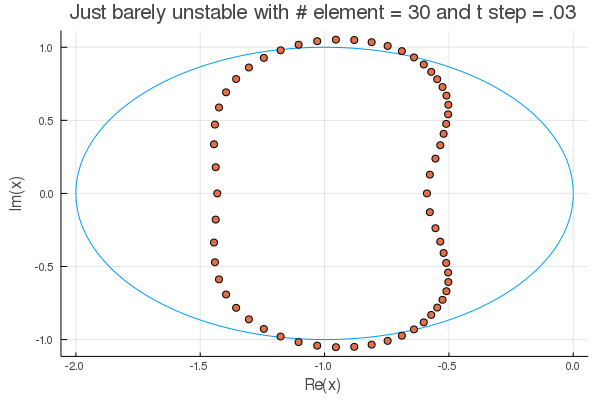
\includegraphics[scale=.5]{barely_unstable.png}

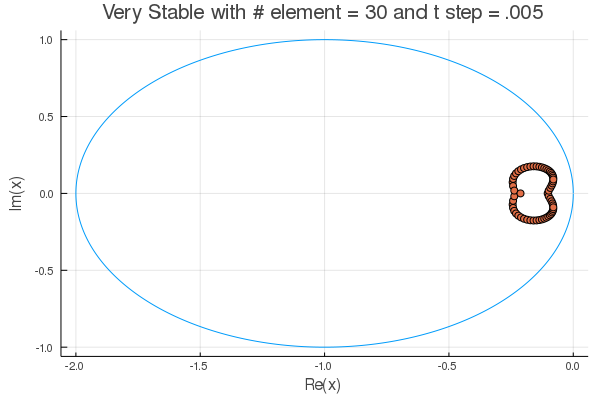
\includegraphics[scale=.5]{very_stable.png}

\section{Convergence Tests}

To test for convergence I found the analytic solution to the problem with:

\begin{gather*}
  u(0, t) = 0 \\
  u(x, 0) = \cos\left(\frac{\pi x}{2}\right) \\
  u(x,t) = \cos\left(\frac{\pi(x - at)}{2}\right)e^{bt}\\
\end{gather*}

\noindent Since each end point of an element is multiply defined, I took the L2 error at each element boundary twice, once for the left element and once for the right. Or as an equation:

$$\text{error} = \sum_{t=0}^T\sum_{i=0}^N (u_{il}^t - u(ih, tk))^2 + (u_{ir}^t - u(ih, tk))^2$$

Here are three plots (where the divergence with many elements should come from the CFL condition):

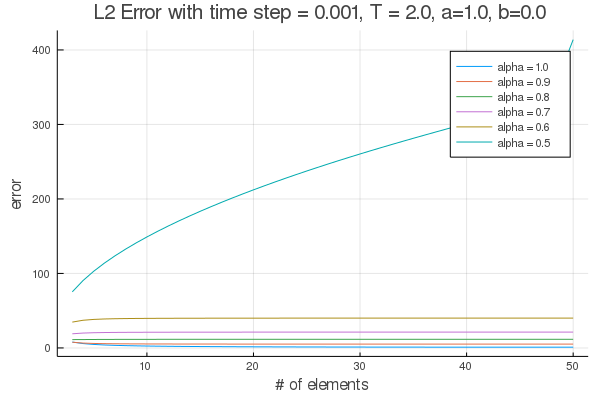
\includegraphics[scale=.5]{compare_alpha.png}

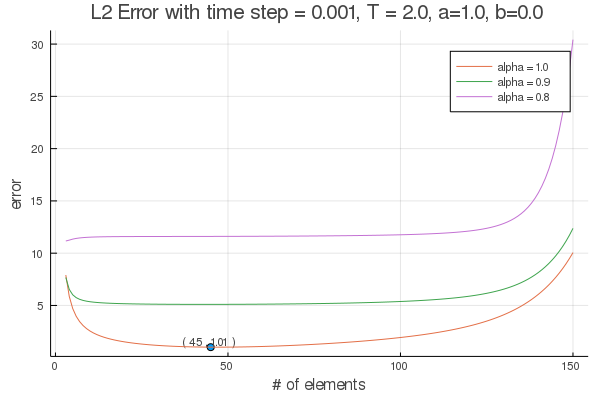
\includegraphics[scale=.5]{upwind_with_best_no_lambda.png}

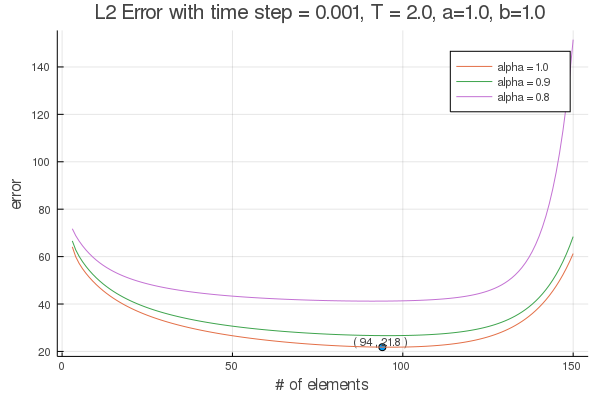
\includegraphics[scale=.5]{upwind_with_best_lambda_1.png}

\newpage


\section{Properties of DG}


Here are a few properties of and thoughts on  DG that make it potentially interesting:

\begin{itemize}
\item Like CG, higher order accuracy can be achieved by increasing number of elements, or by increasing the order of basis functions, but we have the freedom to refine acccuracy element wise with the order of basis functions.
\item capable of modeling physical discontinuities.

\item Parellelizable

\item Can be formulated with only reference to local elements.

\item Why is this better than CG?

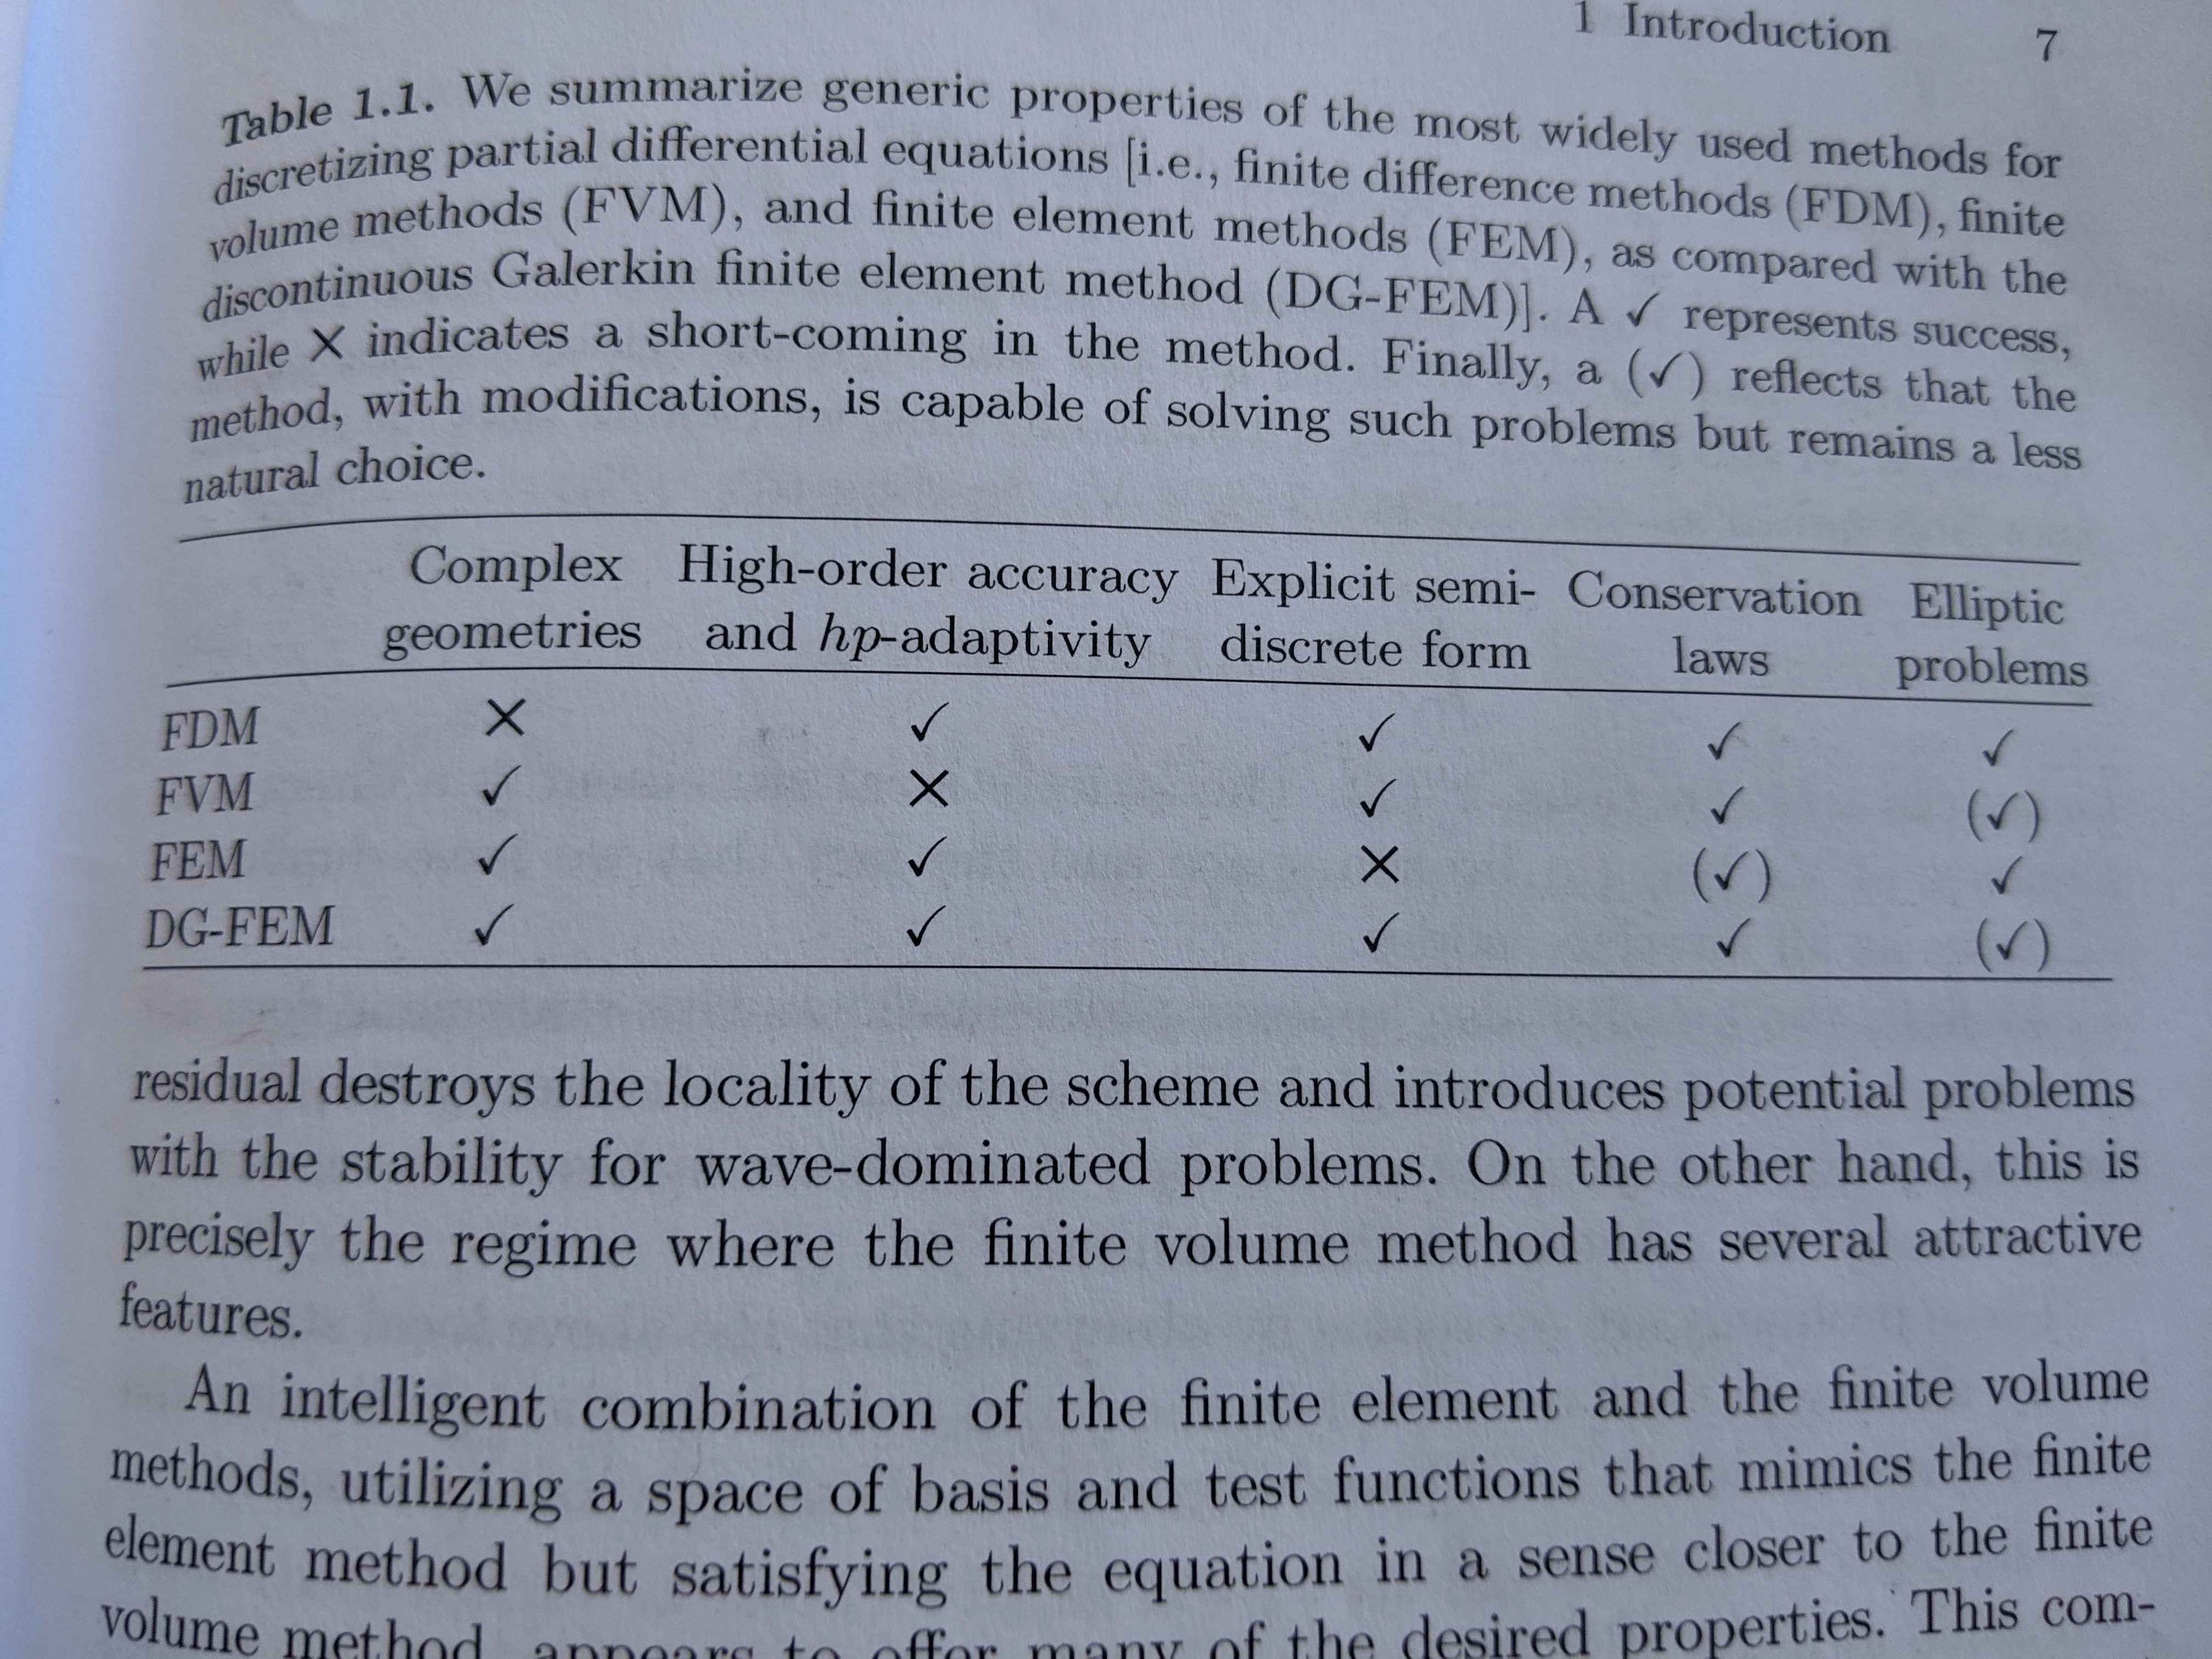
\includegraphics[scale=.5, width=100mm]{table.jpg} 

  
  
\end{itemize}




\end{document}
